\addcontentsline{toc}{section}{Introduction}
\section*{Introduction}
Ce chapitre est dédié à la mise en lumière des pratiques d’architecture logicielle 
employées lors de la conception de notre prototype. 
Nous y présenterons également les choix techniques effectués.

\section{Méthodes de conception}
Dans le souci de décrire de façon fiable, les fonctionnalités du système, nous faisons usage du langage visuel \acrfull{uml}. 
Il s’agit d’une méthode de visualisation d’architecture logicielle permettant de modéliser 
l’architecture logicielle d’un système.

Standardisé par \acrshort{omg}, la version actuelle de \acrshort{uml}, la 2.5 \cite{uml_spec_link}, propose 14 types de diagrammes. 
N'étant pas une méthode, la norme laisse l’utilisation des diagrammes à l'appréciation des utilisateurs.
Dans le cadre de notre prototype, nous avons retenu uniquement les diagrammes de cas d’utilisation, 
de séquence et de classe, car ils expriment bien la structure de notre application.

\subsection{Diagramme de cas d’utilisation}
Les diagrammes de cas d’utilisation illustrent le comportement fonctionnel du système. 
Les cas d’utilisation sont utiles pour décrire les interactions possibles entre 
le/les acteurs acteur(s) et le système.
 
Les acteurs intervenant dans notre système sont:

\begin{itemize}
  \item L’étudiant : il dispose d’un accès en lecture aux informations du système ;
  \item L’enseignant : il dispose d’un accès total en lecture et partiel en écriture sur certaines informations ;
  \item L’administrateur : il dispose de privilèges élevés pour modifier les informations de la plateforme et l’administrer.
\end{itemize}

La figure \ref{fig:use_case_diag} en fait l'illustration.

\begin{figure}[H]
  \centering
  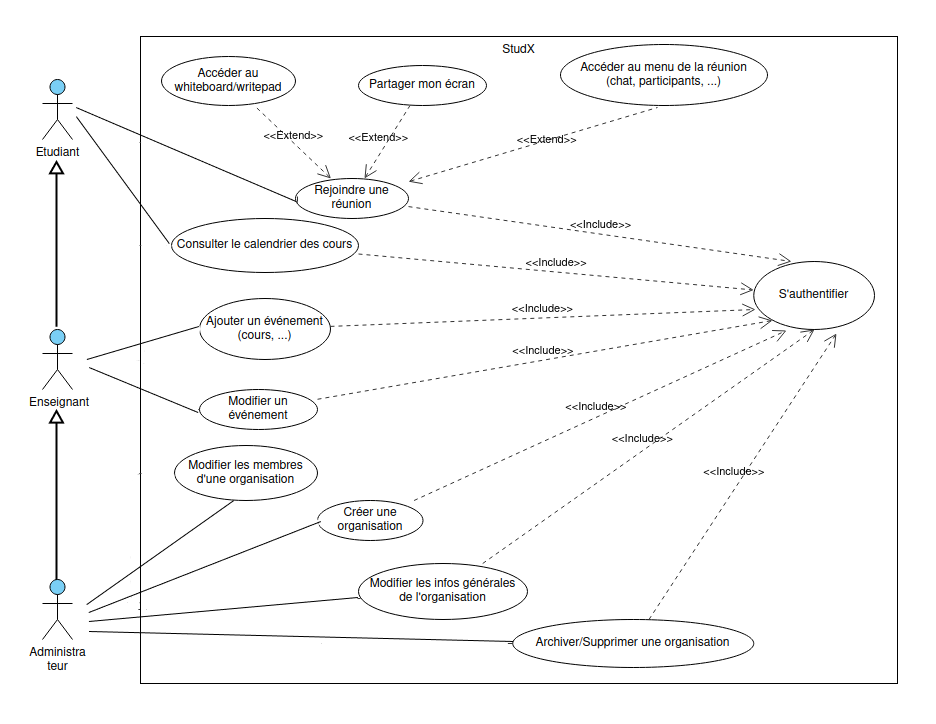
\includegraphics[width=\linewidth]{use-cases-diag}
  \caption{Diagramme de cas d'utilisation du prototype StudX}
  \label{fig:use_case_diag}
\end{figure}


Outre le diagramme, il s'avère parfois nécessaire de fournir, en plus, des descriptions textuelles des cas 
d’utilisation, dans le but d’apporter plus d'éclaircissements. 
Ci-dessous, sont présentées les descriptions textuelles des cas “S’authentifier”, “Ajouter un événement” et “Rejoindre une réunion”.

\subsubsection{Description textuelle du cas d’utilisation “S’authentifier”}
\textbf{Titre} : S’authentifier\newline
\textbf{Objectif} : Authentifier un utilisateur afin qu’il accède à la plateforme\newline
\textbf{Acteurs} : Étudiant ou Enseignant ou Administrateur\newline
\textbf{Pré-conditions} : 
\begin{itemize}[noitemsep,topsep=0pt]
  \item l’utilisateur dispose d’un compte et est admis dans au moins une organisation.
\end{itemize}
\textbf{Séquence nominale} :
\begin{enumerate}[noitemsep,topsep=0pt]
  \item l’utilisateur remplit le formulaire de connexion ;
  \item le système authentifie l’utilisateur ;
  \item le système redirige l’utilisateur vers la page la page d'accueil de l’organisation la plus récente.
\end{enumerate}
\textbf{Post-conditions} : 
\begin{itemize}[noitemsep,topsep=0pt]
  \item l’utilisateur dispose d’une session active.
\end{itemize}
\textbf{Enchaînements alternatifs} :
\begin{itemize}[noitemsep,topsep=0pt]
  \item A1: Identifiants incorrects\newline
    L'enchaînement démarre au point 2.

  \begin{enumerate}[noitemsep,topsep=0pt]
    \setcounter{enumi}{1}
    \item Le système renvoie l’utilisateur vers la page de connexion avec une notification. Ce dernier effectue à nouveau la saisie.
  \end{enumerate}

  \item A2: L’utilisateur n’appartient à aucune organisation.\newline
    L'enchaînement prend départ au point 3.

  \begin{enumerate}[noitemsep,topsep=0pt]
    \setcounter{enumi}{2}
    \item Le système redirige l’utilisateur vers une page 404.
  \end{enumerate}
\end{itemize}


\subsubsection{Description textuelle du cas d’utilisation “Ajouter un événement”}
\textbf{Titre} : Ajouter un événement\newline
\textbf{Objectif} : Planifier les cours en ligne en ajoutant des événements au calendrier\newline
\textbf{Acteurs} : Enseignant ou Administrateur\newline
\textbf{Pré-conditions} : 
\begin{itemize}[noitemsep,topsep=0pt]
  \item l’utilisateur est authentifié en tant qu’enseignant ou administrateur.
\end{itemize}
\textbf{Séquence nominale} :
\begin{enumerate}[noitemsep,topsep=0pt]
  \item L’utilisateur accède au calendrier ;
	\item Le système renvoie les événements actuellement programmes ;
	\item L’utilisateur remplit et soumet un formulaire de création ;
	\item Le système enregistre l'événement et les détails associés ;
	\item Le système notifie les participants concernés.
\end{enumerate}
\textbf{Post-conditions} : 
\begin{itemize}[noitemsep,topsep=0pt]
  \item L’utilisateur accède à l'événement dans son calendrier.
\end{itemize}

\subsubsection{Description textuelle du cas d’utilisation “Rejoindre une réunion”}
\textbf{Titre} : Rejoindre une réunion\newline
\textbf{Objectif} : Tenir une session de classe en ligne\newline
\textbf{Acteurs} : Étudiant ou Enseignant ou Administrateur\newline
\textbf{Pré-conditions} : 
\begin{itemize}[noitemsep,topsep=0pt]
  \item l’utilisateur est authentifié.
\end{itemize}
\textbf{Séquence nominale} :
\begin{enumerate}[noitemsep,topsep=0pt]
  \item  l’utilisateur consulte le calendrier ;
	\item le système affiche les divers événements programmes ;
	\item l’utilisateur accède aux détails d’un événement ;
	\item l’utilisateur clique sur le lien pour rejoindre la reunion ;
	\item le système connecté l’utilisateur aux participants présents.
\end{enumerate}
\textbf{Post-conditions}: 
\begin{itemize}[noitemsep,topsep=0pt]
  \item L’utilisateur est en mesure d’interagir, de communiquer avec les participants.
\end{itemize}

\subsection{Diagramme de séquence}
Le diagramme de séquence décrit les interactions, dans l’espace temps, entre objets dans le cadre des scénarii évoqués au niveau des cas d’utilisations. 
Les figures \ref{fig:auth_seq_diag}, \ref{fig:add_event_seq_diag} et \ref{fig:join_meet_seq_diag} illustrent les diagrammes de séquences pour les trois cas d’utilisation suscités.


\begin{figure}[H]
  \centering
  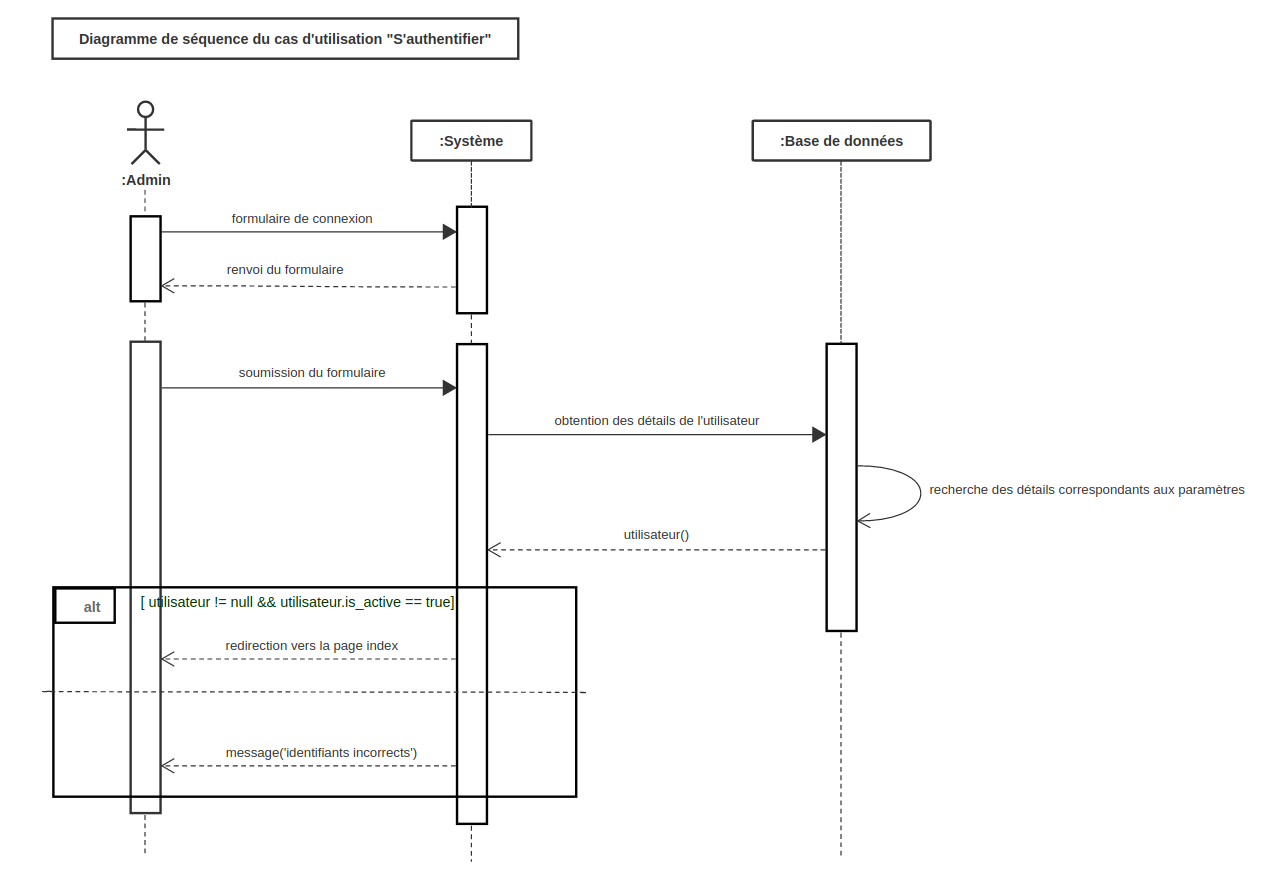
\includegraphics[width=\linewidth]{auth-sequence-diag}
  \caption{Diagramme de séquence du cas d'utilisation “S’authentifier”}
  \label{fig:auth_seq_diag}
\end{figure}

\begin{figure}[H]
  \centering
  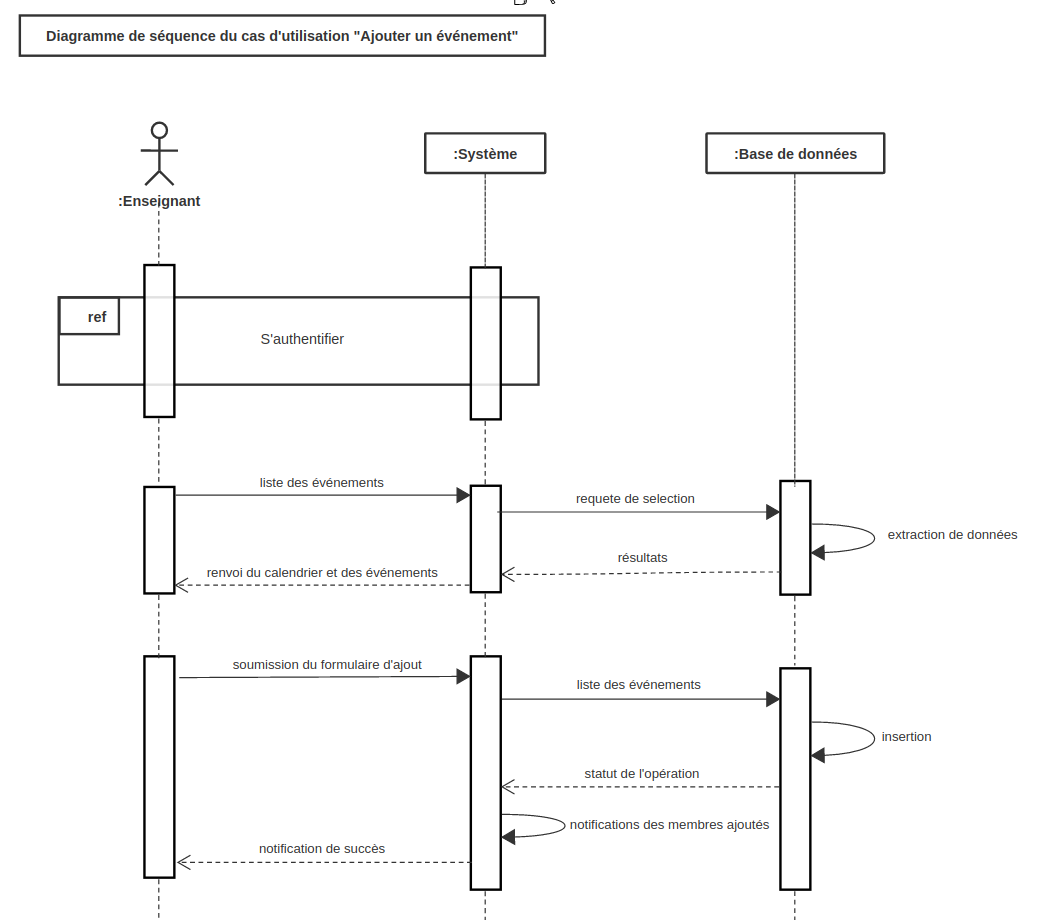
\includegraphics[width=\linewidth]{add-event-sequence-diag}
  \caption{Diagramme de séquence pour le cas d’utilisation “Ajouter un événement”}
  \label{fig:add_event_seq_diag}
\end{figure}

\begin{figure}[H]
  \centering
  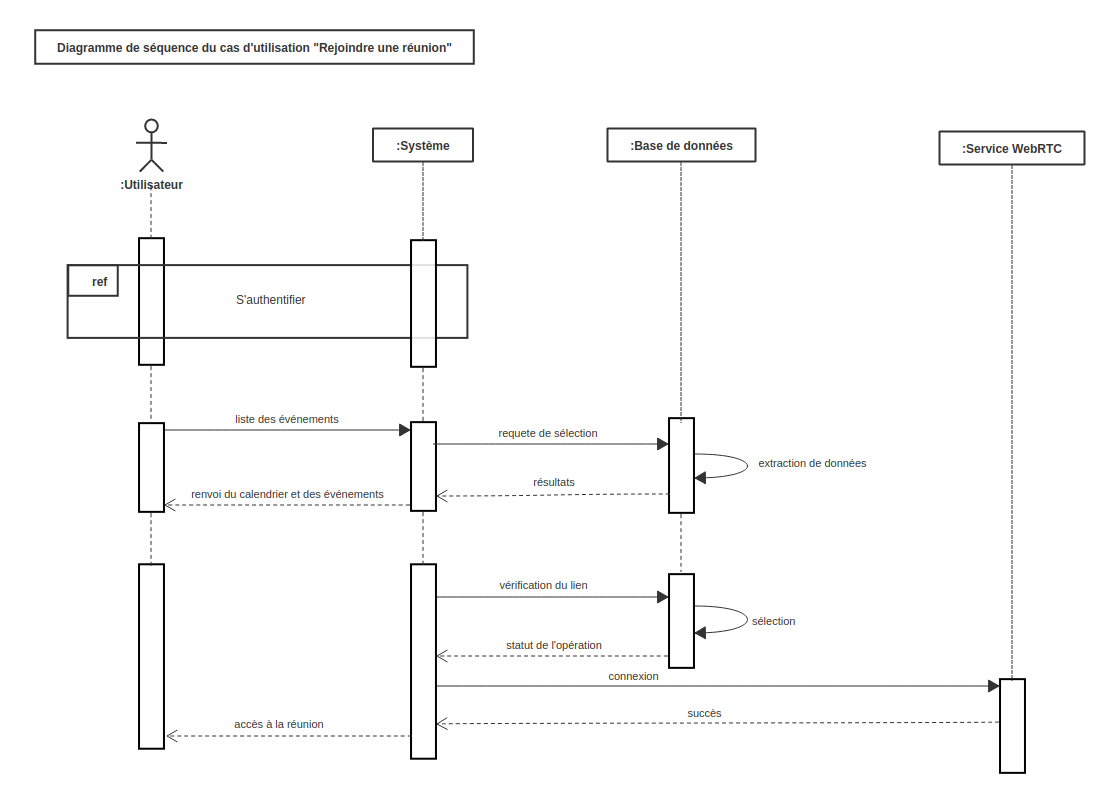
\includegraphics[width=\linewidth]{join-meet-sequence-diag}
  \caption{Diagramme de séquence pour le cas d’utilisation “Rejoindre une réunion”}
  \label{fig:join_meet_seq_diag}
\end{figure}

\subsection{Diagramme de classe}
Le diagramme de classe illustre les classes et les interfaces du système ainsi que les relations qui les lient. 
Le diagramme à la figure \ref{fig:class_diag} en dessous décrit les diverses entités de notre prototype.

\begin{figure}[H]
  \centering
  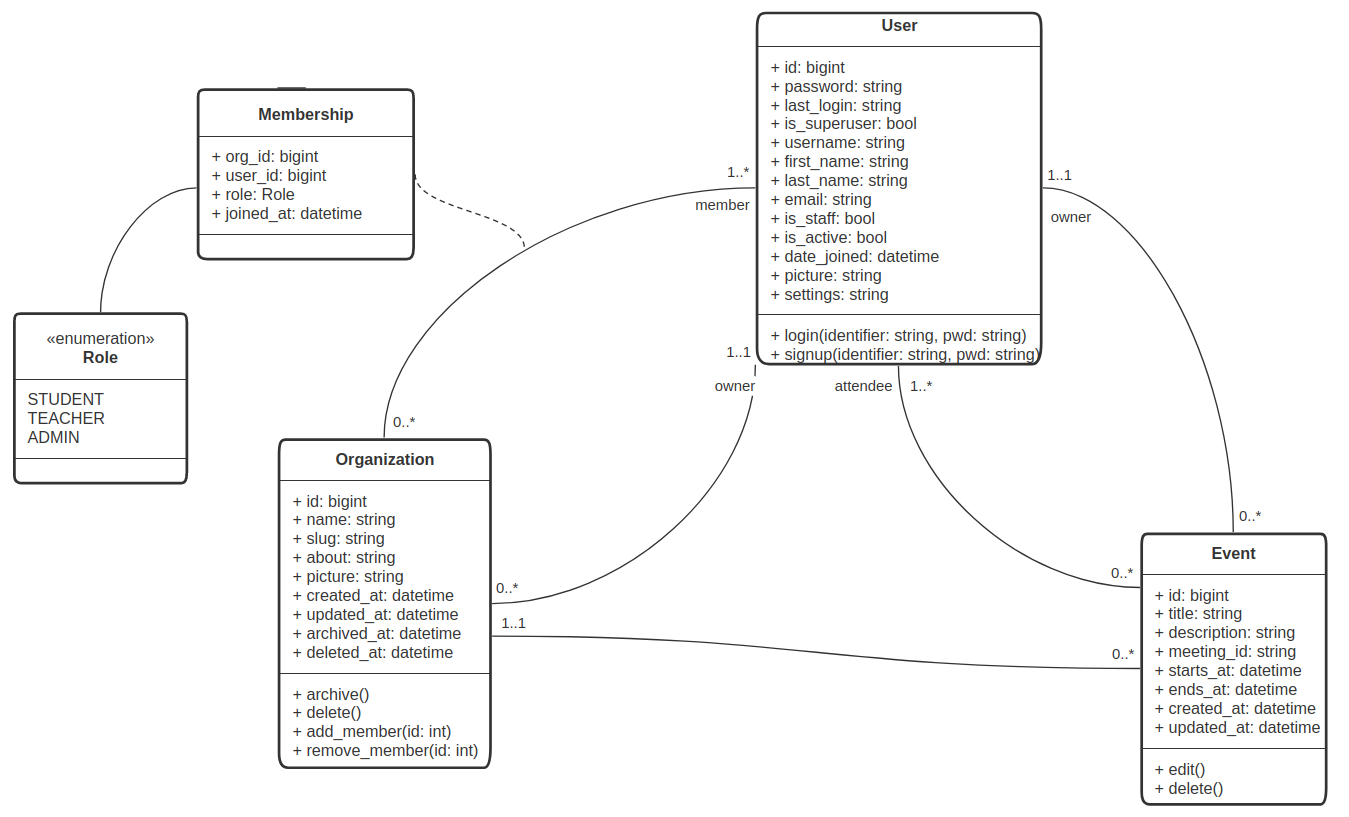
\includegraphics[width=\linewidth]{class-diag}
  \caption{Diagramme de classe}
  \label{fig:class_diag}
\end{figure}

\subsection{Architecture du système}
Pour assurer la scalabilité des systèmes, il est important de bien en concevoir l’architecture. 
Dans ce but, nous avons adopté une approche découplée, isolant les composantes du système. 
Il s’agit de microservices. Toutefois, il est important de noter qu'à l'échelle d’un prototype, 
l’architecture proposée reste très simplifiée et ne prend pas en compte des facteurs comme la résilience \cite{microservices_resiliency}. 
La figure de l'encart \ref{fig:system_design} présente les diverses composantes de notre architecture.


\begin{figure}[H]
  \centering
  \frame{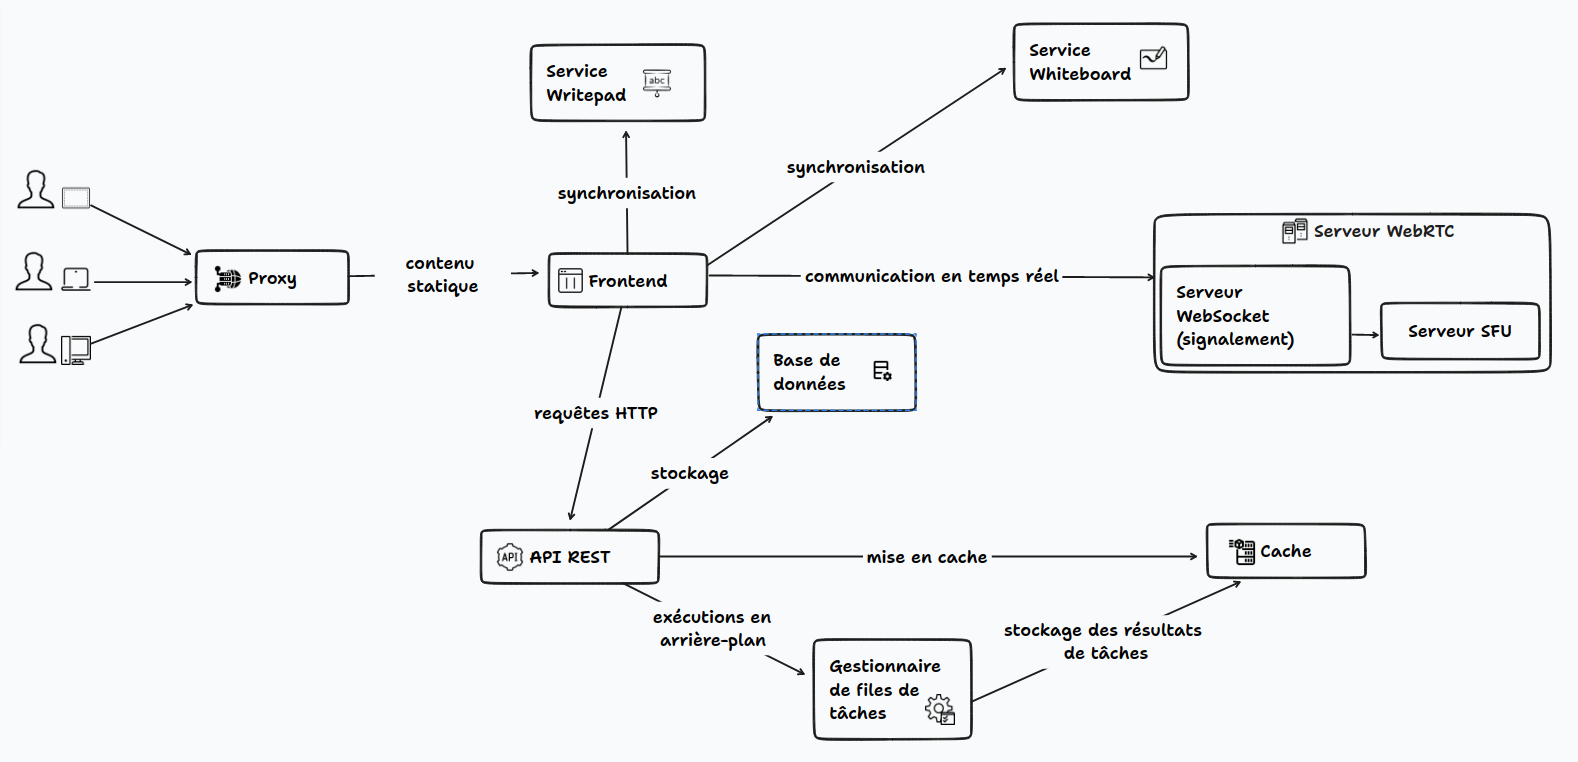
\includegraphics[width=\linewidth]{studx-system-design}}
  \caption{Architecture du système du prototype StudX}
  \label{fig:system_design}
\end{figure}

On peut notamment remarquer que toutes les interactions entre le système et les utilisateurs passent toutes par un proxy. 
Ceci s’explique principalement par la volonté d'éviter les problèmes de CORS, 
qui occurrent dès lors que les services ne sont pas tous sur un même domaine.

Outre ces détails, il faut préciser également que le prototype implémente l’architecture de multi-entité \cite{multitenancy}, 
en regroupant les utilisateurs et les données qui leur sont communes en entités que nous qualifions d’organisation. 
Le but est de pouvoir servir plusieurs regroupements sans pour autant avoir à répliquer le matériel. 

\section{Matériels}
\subsection{Choix techniques}
Faisant référence à l’architecture suscitée, 
voyons à présent les technologies employées dans la mise en place de la solution.

\subsubsection{Proxy}
Un serveur proxy sert de relais entre différentes parties, notamment entre le client et le serveur dans notre contexte. 
Il s’agit dans ce cas, d’un reverse proxy, car le relai va du client vers le serveur.
 
\textbf{Caddy} est un serveur Web moderne qui offre un large panel de fonctionnalités. 
Il offre un large éventail de fonctionnalités que l’on peut mettre en place via un fichier de configuration spéciale nommé Caddyfile. 
La figure \ref{fig:caddyfile} en présente un exemple, extrait du code de notre prototype.


\begin{figure}[H]
  \centering
  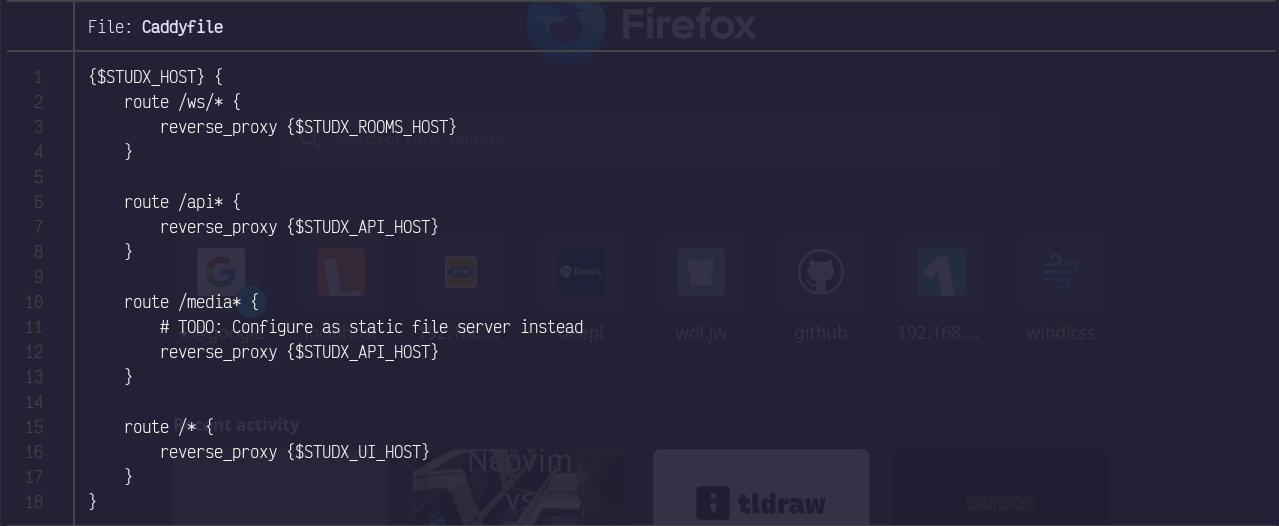
\includegraphics[width=\linewidth]{caddyfile}
  \caption{Example de configuration du proxy \textbf{Caddy}}
  \label{fig:caddyfile}
\end{figure}

On peut remarquer entre autres, l’utilisation de variables d’environnement qui permettent de rendre la configuration encore plus dynamique. 
Tous ces atouts en font un bon choix pour notre prototype.

\subsubsection{API REST}

Une \acrshort{api} \acrshort{rest} définit interface de programmation respectant les contraintes du style d’architecture \acrlong{rest}.

Elle doit disposer des caractéristiques suivantes :

\begin{itemize}
  \item Une architecture client-serveur constituée de clients, de serveurs et de ressources, avec des requêtes gérées via \acrshort{http} ;
  \item Des communications client-serveur sans etat, c'est-à-dire que les informations du client ne sont jamais stockées entre les requêtes, 
  qui doivent être traitées séparément, de manière totalement indépendante ;
  \item La possibilité de mettre en cache des données afin de rationaliser les interactions client-serveur ;
  \item Une interface uniforme entre les composants qui permet un transfert standardisé des informations ;
  \item Un système à couches, invisible pour le client, qui permet de hiérarchiser les différents types de serveurs 
  (pour la sécurité, l'équilibrage de charge, etc.) impliqués dans la récupération des informations demandées ;
  \item Du code à la demande (facultatif), c'est-à-dire la possibilité d'envoyer du code exécutable depuis le serveur vers le client 
  (lorsqu'il le demande) afin d'étendre les fonctionnalités d'un client.\cite{redhat_rest_spec}
\end{itemize}

Pour ce faire, notre choix s’est porté sur \textbf{Django}, un framework du langage \textbf{Python} offrant une facilité de conception grâce aux nombreuses fonctionnalités déjà incluses par défaut. 
Avec l’emploi de modules comme \textbf{Django Rest Framework}, il est possible de concevoir une \acrshort{api} totalement conforme aux recommandations de la spécification \acrshort{rest}.

\begin{figure}[H]
  \centering
  
\includegraphics[width=0.25\linewidth]{django-logo-positive}
  \caption{Logo du framework \textbf{Django}}
  \label{fig:django_logo}
\end{figure}


\subsubsection{Frontend}
La conception de l’interface utilisateur a nécessité l’usage des langages \acrshort{html}, \acrshort{css} et \textbf{Typescript}.

\acrshort{html} est un langage de balisage standardisé, qui permet la conception de documents Web. 
Assisté du langage de style \acrshort{css}, il est possible de concevoir une mise en page attrayante favorisant l'expérience utilisateur.

\textbf{Typescript} est un langage conçu au-dessus du langage \textbf{JavaScript}. 
Il vise notamment à améliorer ce dernier en fournissant un système de typage fort. 
Cela permet entre autres de réduire le nombre de bugs qui finissent en production et d'améliorer l'expérience du développeur.

Afin de faciliter l'intégration de tous les outils suscités, nous avons fait recours au framework \textbf{Vue.js}. 
\textbf{Vue} est un framework moderne de conception d’application Web qui se concentre sur le rendu déclaratif et composition de composants. 
Des solutions complémentaires maintenues officiellement, permettent la gestion du routage, de l'état et bien d’autres fonctionnalités comme les \acrshort{pwa}s. 
Au vu des avantages qu’il présente, il correspond parfaitement aux besoins de notre plateforme en termes d’interfaces.

\begin{figure}[h]
  \centering
  
\includegraphics[width=0.25\linewidth]{vue-logo}
  \caption{Logo du framework \textbf{Vue.js}}
  \label{fig:vue_logo}
\end{figure}


\subsubsection{Base de données}
Les systèmes de gestion de bases de données sont des éléments clés dans la conception d’applications dynamiques. 
Elles permettent le stockage, le filtrage, la mise à jour et la suppression des données du système. 
On distingue généralement deux grandes familles de base de données: les bases relationnelles et les bases non relationnelles. 
La première préconise l’utilisation d’un schéma fixe représentant la structure de la donnée alors que le seconde permet une flexibilité du schéma et autorise l’insertion de colonnes quelconques.

Notre choix s’est porté vers PostgreSQL, un système de gestion de base de données relationnel. 
C’est d’ailleurs, le seul système Open Source, fournissant des fonctionnalités dignes de concurrencer les maisons d'édition comme Oracle.

\begin{figure}[H]
  \centering
  
\includegraphics[width=0.2\linewidth]{postgresql-logo}
  \caption{Logo de \textbf{PostgreSQL}}
  \label{fig:pg_logo}
\end{figure}

\subsubsection{Gestionnaire de files de tâches}
Effectuer des tâches qui demandent des ressources intensives lors de requêtes \acrshort{http}, risque d’en dégrader les performances. 
Pour éviter celà, nous avons recours à \textbf{Celery}, un gestionnaire de files de tâches moderne qui offre une intégration quasi-parfaite avec le framework \textbf{Django}.

\textbf{Celery} supporte un large panel de protocoles de communication pour la planification des tâches et la récupération des résultats. 
Pour simplifier l’architecture, nous nous sommes servi du cache comme relai afin de déclencher des tâches.


\begin{figure}[H]
  \centering
  
\includegraphics[width=0.25\linewidth]{celery-logo}
  \caption{Logo de \textbf{Celery}}
  \label{fig:celery_logo}
\end{figure}


\subsubsection{Cache}
En architecture logicielle, le cache est une composante essentielle. 
Il permet d'améliorer les performances du système en gardant une copie 
(en mémoire, à court terme) des données auxquelles les utilisateurs ont précédemment accédé,
sans qu’il n’y ait besoin de reprendre le même processus de traitement de la requête. 
Ceci réduit le temps de réponse mais aussi réduit la pression sur toute l’infrastructure. 
La base de données est moins sollicitée par exemple. Nous avons opté pour Redis, 
une solution Open Source qui utilise la mémoire vive de la machine pour permettre un accès en lecture 
et en écriture très très rapide.


\begin{figure}[H]
  \centering
  
\includegraphics[width=0.25\linewidth]{redis-logo}
  \caption{Logo de \textbf{Redis}}
  \label{fig:redis_logo}
\end{figure}

\subsubsection{Service Writepad}
Dans le cadre de la conception d’un service synchronisé d'écriture, nous avons employé l'éditeur populaire \textbf{TipTap}. 
Il s’agit d’un éditeur Open Source offrant un large panel de fonctionnalités dont la collaboration entre utilisateurs. 
Grâce à une documentation extensive, il est d’autant plus facile de l'intégrer à une application.

\begin{figure}[H]
  \centering
  
\includegraphics[width=0.2\linewidth]{tiptap-logo-version}
  \caption{Logo de \textbf{TipTap} et version actuelle}
  \label{fig:tiptap_logo_and_version}
\end{figure}

\subsubsection{Service Whiteboard}
Le service Writepad est le clone d’un projet Open source sous licence MIT, dénommé \textbf{whiteboard}. 
Il est consultable a l’adresse URL suivante: \href{https://github.com/cracker0dks/whiteboard}{https://github.com/cracker0dks/whiteboard}. 
Les modifications effectuées touchent principalement l’interface utilisateur mais aussi font omission de fonctionnalités qui ne nous intéressent pas à l'état actuel du prototype. 
La figure de l’encart \ref{fig:whiteboard_demo} en présente l’interface par défaut.


\begin{figure}[H]
  \centering
  \frame{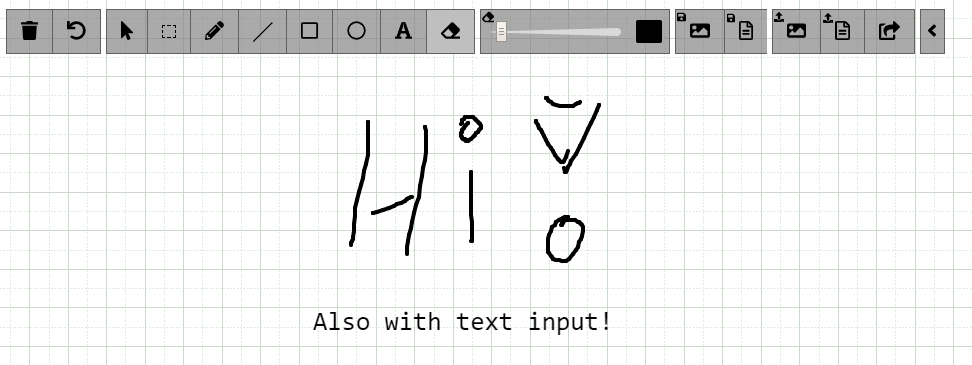
\includegraphics[width=0.75\linewidth]{whiteboard-upstream-demo}}
  \caption{Interface par défaut de \textbf{whiteboard}}
  \label{fig:whiteboard_demo}
\end{figure}


\subsubsection{Serveur WebRTC}
\textbf{Rust} est un langage compilé qui se veut performant, sûr et productif\cite{rust}. 
Le langage peut notamment donner des garanties d'absence d'erreur de segmentation ou de situation de concurrence 
dès l'étape de compilation. De plus, ceci se fait sans ramasse-miettes. Ses performances sont comparables à celles du \textbf {C} ou du \textbf{C++} pour ce qui concerne la vitesse d'exécution. 
Tout cela en fait un choix excellent pour le développement d'applications de réseau. Parmi les solutions Open Source pour la mise en place d’un serveur \acrshort{webrtc}, 
nous avons opté pour \textbf{Mediasoup}. C’est un serveur de relai \acrshort{sfu} qui offre une bibliothèque \textbf{Rust} pour l'intégration dans diverses catégories d'applications. 

\textbf{Actix} est un framework reposant sur le modèle d’acteurs \cite{actor_design_pattern} et écrit en \textbf{Rust}. 
Il offre un framework web (\textbf{actix-web}) qui permet d’implémenter des services web reposant sur le modèle d’acteurs. 
C’est un framework toutes batteries incluses qui supporte nativement bien de fonctionnalités comme le support des Websockets, lu protocole \acrshort{tls} ou encore de la version 2 du protocole \acrshort{http} (HTTP/2). 
Il offre d’excellentes performances, raison pour laquelle nous l’avons choisi, pour la gestion du signalement lors des connexions \acrshort{webrtc}.

Ci-dessous est un extrait du code source de notre prototype \textbf{StudX}, qui présente la syntaxe du langage \textbf{Rust},  et montre l'intégration des divers outils suscités:
\inputminted{rust}{2-partie/main.rs}

\subsection{Outils de développement}
Le tableau \ref{table:dev_tools} présente une liste non exhaustive des outils de développement employés pour la réalisation du prototype.

\begin{table}[H]
  \centering
\begin{tabular}{|l|l|l|}
  \hline
  \multicolumn{3}{|c|}{Outils de développement} \\
  \hline
  \multicolumn{3}{|c|}{Matériel} \\
  \hline
  Nom & \multicolumn{2}{c|}{Description} \\
  \hline
  Laptop Acer ES1-521 & \multicolumn{2}{l|}{Employé pour les tests de la solution} \\
  \hline
  Laptop Lenovo Thinkbook & \multicolumn{2}{l|}{Employé pour le développement et les tests} \\
  \hline
  Smartphone TECNO Spark 8C & \multicolumn{2}{l|}{Smartphone pour les besoins de tests d'accessibilité} \\
  \hline
  Routeur ZTE MF927U & \multicolumn{2}{l|}{Mise en réseau des appareils} \\
  \hline
  \multicolumn{3}{|c|}{Systèmes d'exploitation} \\
  \hline
  Nom & \multicolumn{2}{l|}{Version} \\
  \hline
  Manjaro Linux & \multicolumn{2}{l|}{22.0.4} \\
  \hline
  Fedora & \multicolumn{2}{l|}{36} \\
  \hline
  \multicolumn{3}{|c|}{Logiciels} \\
  \hline
  Nom & Description & Version \\
  \hline
  \acrshort{edi} Jetbrains & \makecell{Suite de développement logiciel} & \makecell{Versions \textbf{Pro} de \\ Pycharm, \\ CLion et \\ WebStorm} \\
  \hline
  neovim & \makecell{Editeur de texte modal} & 0.8 \\
  \hline
  Git, GitHub & Versionnement de code source & \textit{git}: 2.39.2 \\
  \hline
  Docker & \makecell{Outil de conteneurisation d’applications} & 23.0.1 \\
  \hline
\end{tabular}
\caption{Liste non exhaustive des outils employés dans la réalisation de \textbf{StudX}}
\label{table:dev_tools}
\end{table}

\addcontentsline{toc}{section}{Conclusion}
\section*{Conclusion}
Ce chapitre a permis de passer en revue les choix de conception ainsi que les choix techniques effectués
pour la mise en œuvre de notre prototype d’application. 
Ceci pose des fondations robustes à l'implémentation de ladite solution. En suivant les décisions techniques prises, 
nous avons construit notre prototype. 
Le but du chapitre suivant sera de le présenter puis de faire un bilan d'évaluation.
